% Titre de la premiere partie
\section{Introduction Historique}

%%%%%%%%%%%%%%%%%%%%%%%%%%%%%%%%%%%%%%%%%%%%%%%%
% Première diapo
%%%%%%%%%%%%%%%%%%%%%%%%%%%%%%%%%%%%%%%%%%%%%%%%
\begin{frame}
\frametitle{Contexte scientifique }
\framesubtitle{Premiers modèles}

Craig Reynolds (1987) : Premier modèle de mouvement de foule : les boids


\begin{itemize}
	\item	<2->	Représentation de nuées d’oiseaux
	\item	<3->	Règles très simples
	\item   <4->      Vitesses et trajectoires des agents liées aux voisins proches

	\visible<5->{
	\begin{figure}
	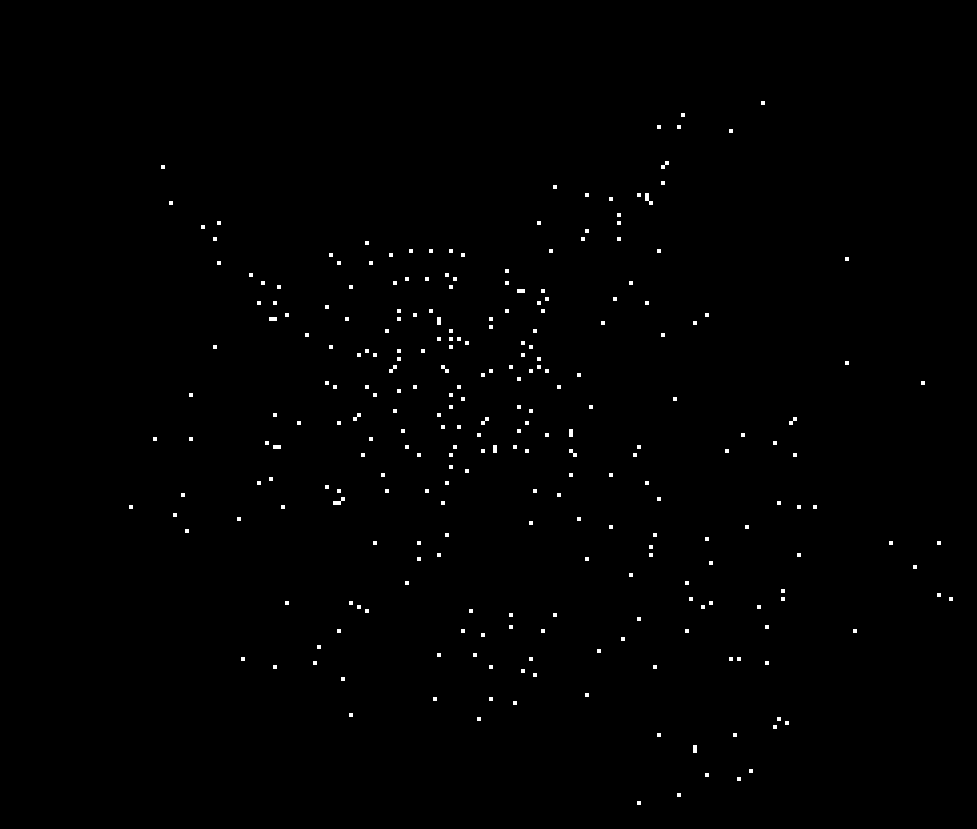
\includegraphics[width=0.5\linewidth]{figures/Fig01}
	\end{figure}
	}
	
\end{itemize}

\end{frame}


%%%%%%%%%%%%%%%%%%%%%%%%%%%%%%%%%%%%%%%%%%%%%%%%
% Deuxième diapo
%%%%%%%%%%%%%%%%%%%%%%%%%%%%%%%%%%%%%%%%%%%%%%%%
\begin{frame}
\frametitle{Introduction historique}
\framesubtitle{Premiers modèles}

% AFFICHAGE PAS TERRIBLE ICI
Dirk Helbing et Péter Molnar (1998) : Le concept de "forces sociales"


\begin{itemize}
	\item	<2->	Force d’attraction sociale : les trajectoires peuvent être influencées

	\item	<3->	Force de répulsion : les contacts physiques sont évités
 \end{itemize}
\bigskip
\onslide<4-> Julien Pettre et Wouter Van Toll (2021) : Evitement de collision

 \begin{itemize}
     \item <5-> Les trajectoires sont adoucies et plus réalistes en fonction des obstacles
 \end{itemize}	

\end{frame}


%%%%%%%%%%%%%%%%%%%%%%%%%%%%%%%%%%%%%%%%%%%%%%%%
% Troisième diapo
%%%%%%%%%%%%%%%%%%%%%%%%%%%%%%%%%%%%%%%%%%%%%%%%
%\begin{frame}
%\frametitle{Introduction historique}
%\framesubtitle{Modèles plus réalistes}
%
%Bertrand Maury/Juliette Venel (2009) : Modèle plus réaliste
%
%\begin{itemize}
%	\item	<1->	Agents représentés par des cercles (pas de chevauchement)
%    \item <2-> Forces de répulsion
%	\item	<3-> Prédiction de mouvement
%\end{itemize}
%\end{frame}


%%%%%%%%%%%%%%%%%%%%%%%%%%%%%%%%%%%%%%%%%%%%%%%%
% Quatrième diapo
%%%%%%%%%%%%%%%%%%%%%%%%%%%%%%%%%%%%%%%%%%%%%%%%
\begin{frame}
\frametitle{Introduction historique}
\framesubtitle{Modèles plus réalistes}


\visible<1->{
	\begin{figure}
	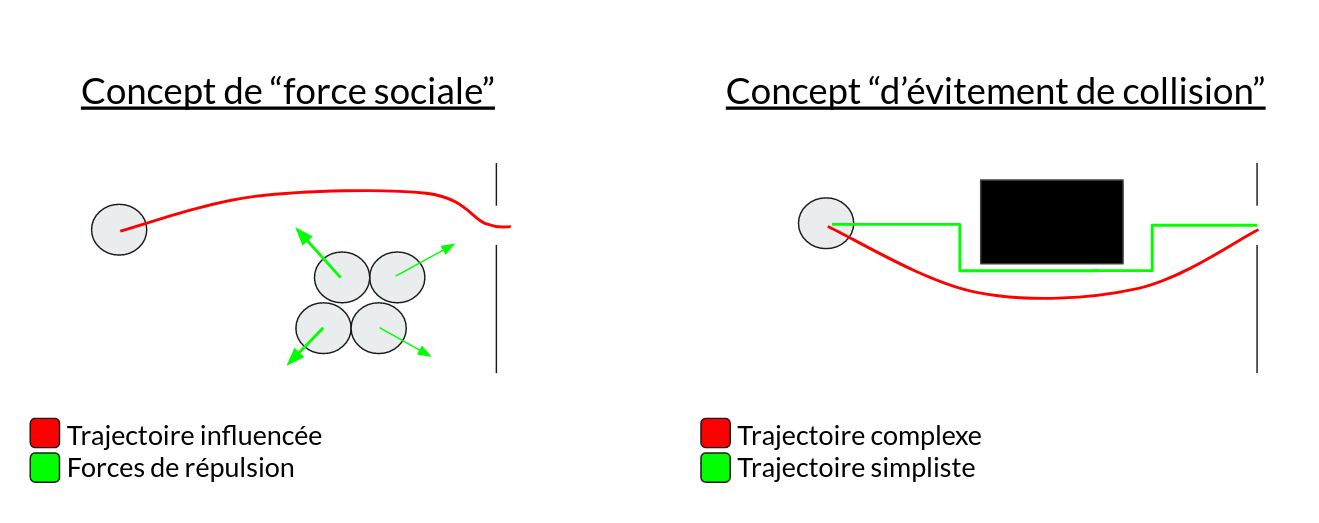
\includegraphics[width=1\linewidth]{figures/Fig02}
	\end{figure}
}
 
\end{frame}
